\documentclass{article}
\usepackage{amsmath}
\usepackage{amssymb}
\usepackage{tikz}
\usetikzlibrary{calc,patterns,arrows.meta}

\begin{document}

\section*{Campo elettrico di 4 cariche\\ai vertici di un quadrato}

\subsection*{1. Configurazione del sistema e coordinate dei vertici}

Consideriamo quattro cariche puntiformi uguali di modulo $q$ disposte ai vertici di un quadrato di lato $l$ centrato nell'origine del piano $xy$, con lati paralleli agli assi.

I quattro vertici hanno coordinate:
\begin{align*}
V_1 &= \left(\frac{l}{2}, \frac{l}{2}, 0\right), \quad &V_2 = \left(-\frac{l}{2}, \frac{l}{2}, 0\right) \\
V_3 &= \left(-\frac{l}{2}, -\frac{l}{2}, 0\right), \quad &V_4 = \left(\frac{l}{2}, -\frac{l}{2}, 0\right)
\end{align*}

Vogliamo calcolare il campo elettrico generato dalle cariche in un punto generico $P = (x, 0, 0)$ situato lungo l'asse $x$.

\begin{figure}[htbp]
\centering
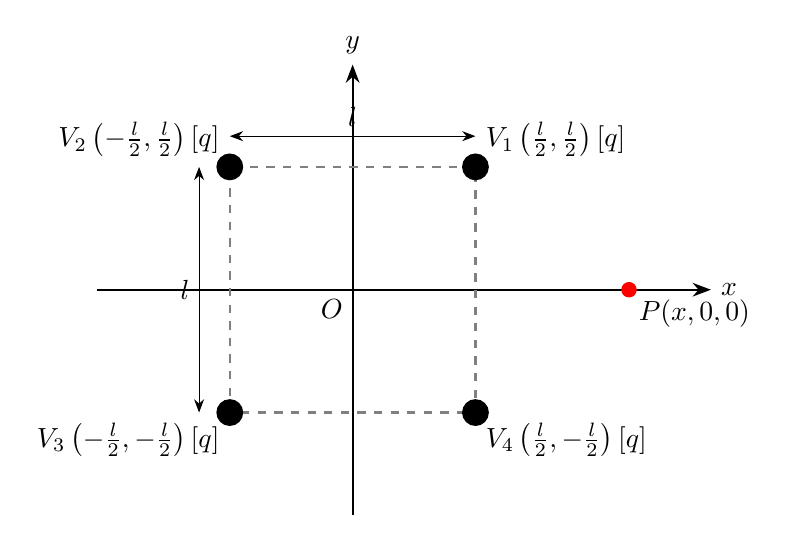
\begin{tikzpicture}[scale=1.3, >=Stealth]
    % Assi cartesiani
    \draw[->, thick] (-2.5,0) -- (3.5,0) node[right] {$x$};
    \draw[->, thick] (0,-2.2) -- (0,2.2) node[above] {$y$};
    \node[below left] at (0,0) {$O$};

    % Quadrato
    \draw[dashed, thick, color=gray] (-1.2,-1.2) rectangle (1.2,1.2);

    % Quote del lato
    \draw[<->] (-1.2,1.5) -- (1.2,1.5) node[midway, above] {$l$};
    \draw[<->] (-1.5,-1.2) -- (-1.5,1.2) node[midway, left] {$l$};

    % Cariche ai vertici
    \filldraw[fill=black!100, draw=black!100!black, thick] (1.2,1.2) circle (0.12) node[above right] {$V_1\left(\frac{l}{2}, \frac{l}{2}\right) [q]$};
    \filldraw[fill=black!100, draw=black!100!black, thick] (-1.2,1.2) circle (0.12) node[above left] {$V_2\left(-\frac{l}{2}, \frac{l}{2}\right) [q]$};
    \filldraw[fill=black!100, draw=black!100!black, thick] (-1.2,-1.2) circle (0.12) node[below left] {$V_3\left(-\frac{l}{2}, -\frac{l}{2}\right) [q]$};
    \filldraw[fill=black!100, draw=black!100!black, thick] (1.2,-1.2) circle (0.12) node[below right] {$V_4\left(\frac{l}{2}, -\frac{l}{2}\right) [q]$};

    % Punto P sull'asse x
    \filldraw[red] (2.7,0) circle (0.07) node[below right, color=black] {$P(x,0,0)$};
\end{tikzpicture}
\caption{Disposizione delle cariche $q$ ai vertici del quadrato di lato $l$ e punto di osservazione $P(x,0,0)$.}
\end{figure}

\subsection*{2. Contributo della coppia di destra ed elisione delle componenti ortogonali}

Valutiamo il contributo delle cariche $V_1$ e $V_4$ poste sul lato destro ($x = l/2$). La distanza $r_d$ di ciascuna delle due cariche dal punto $P(x,0,0)$ vale:
\begin{equation*}
r_d = \sqrt{\left(x - \frac{l}{2}\right)^2 + \left(\frac{l}{2}\right)^2}
\end{equation*}

Per simmetria speculare rispetto all'asse $x$, le componenti $y$ dei due campi generati da $V_1$ e $V_4$ sono uguali e opposte, quindi si annullano. Resta soltanto la componente lungo $x$:
\begin{equation*}
E_{x,\text{destra}}(x) = 2 \cdot \frac{q}{4\pi\varepsilon_0 r_d^2} \cos\theta_d = \frac{2q}{4\pi\varepsilon_0} \frac{x - \frac{l}{2}}{\left[\left(x - \frac{l}{2}\right)^2 + \frac{l^2}{4}\right]^{3/2}}
\end{equation*}

\begin{figure}[htbp]
\centering
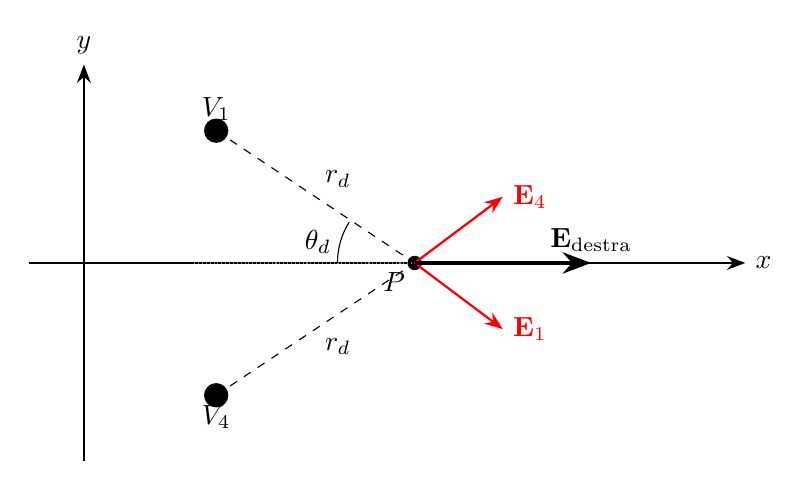
\begin{tikzpicture}[scale=1.4, >=Stealth]
    % Assi
    \draw[->, thick] (-0.5,0) -- (6,0) node[right] {$x$};
    \draw[->, thick] (0,-1.8) -- (0,1.8) node[above] {$y$};

    % Cariche destra
    \filldraw[fill=black!100, draw=black!100!black, thick] (1.2,1.2) circle (0.1) node[above] {$V_1$};
    \filldraw[fill=black!100, draw=black!100!black, thick] (1.2,-1.2) circle (0.1) node[below] {$V_4$};

    % Punto P
    \coordinate (P) at (3,0);
    \filldraw[black] (P) circle (0.06) node[below left] {$P$};

    % Vettori raggio
    \draw[dashed] (1.2,1.2) -- (P) node[midway, above right] {$r_d$};
    \draw[dashed] (1.2,-1.2) -- (P) node[midway, below right] {$r_d$};

    % Vettori campo
    \draw[->, red, thick] (P) -- ($(P) + (0.8, -0.6)$) node[right] {$\mathbf{E}_1$};
    \draw[->, red, thick] (P) -- ($(P) + (0.8, 0.6)$) node[right] {$\mathbf{E}_4$};
    \draw[->, black, ultra thick] (P) -- ($(P) + (1.6, 0)$) node[above] {$\mathbf{E}_{\text{destra}}$};

    % Angolo theta
    \draw[gray, densely dotted] (1,0) -- (P);
    \draw (2.3,0) arc (180:148:0.7) node[midway, left] {$\theta_d$};
\end{tikzpicture}
\caption{Composizione dei vettori di campo generati dalla coppia di cariche del lato destro.}
\end{figure}

\subsection*{3. Contributo della coppia di sinistra e campo risultante}

In modo del tutto analogo, per la coppia di cariche sul lato sinistro ($V_2$ e $V_3$, poste a $x = -l/2$), la distanza dal punto $P$ è:
\begin{equation*}
r_s = \sqrt{\left(x + \frac{l}{2}\right)^2 + \left(\frac{l}{2}\right)^2}
\end{equation*}

Anche in questo caso le componenti ortogonali si annullano, fornendo la sola componente $x$:
\begin{equation*}
E_{x,\text{sinistra}}(x) = \frac{2q}{4\pi\varepsilon_0} \frac{x + \frac{l}{2}}{\left[\left(x + \frac{l}{2}\right)^2 + \frac{l^2}{4}\right]^{3/2}}
\end{equation*}


\begin{figure}[htbp]
\centering
\begin{tikzpicture}[scale=1.4, >=Stealth]
    % Assi
    \draw[->, thick] (-0.5,0) -- (6,0) node[right] {$x$};
    \draw[->, thick] (0,-1.8) -- (0,1.8) node[above] {$y$};

    % Cariche sx
    \filldraw[fill=black!100, draw=black!100!black, thick] (-1.2,1.2) circle (0.1) node[above] {$V_2$};
    \filldraw[fill=black!100, draw=black!100!black, thick] (-1.2,-1.2) circle (0.1) node[below] {$V_3$};

    % Punto P
    \coordinate (P) at (3,0);
    \filldraw[black] (P) circle (0.06) node[below left] {$P$};

    % Vettori raggio
    \draw[dashed] (-1.2,1.2) -- (P) node[midway, above right] {$r_s$};
    \draw[dashed] (-1.2,-1.2) -- (P) node[midway, below right] {$r_s$};

    % Vettori campo
    \draw[->, red, thick] (P) -- ($(P) + (0.6, -0.3)$) node[below right] {$\mathbf{E}_2$};
    \draw[->, red, thick] (P) -- ($(P) + (0.6, 0.3)$) node[above right] {$\mathbf{E}_3$};
    \draw[->, black, ultra thick] (P) -- ($(P) + (1.2, 0)$) node[above] {$\mathbf{E}_{\text{sinistra}}$};

    % Angolo theta
    \draw[gray, densely dotted] (1,0) -- (P);
    \draw (2.3,0) arc (180:164:0.7) node[midway, left] {$\theta_s$};
\end{tikzpicture}
\caption{Composizione dei vettori di campo generati dalla coppia di cariche del lato destro.}
\end{figure}



Sommando i contributi vettoriali, l'espressione analitica finale del campo elettrico in funzione della posizione $x$ sull'asse risulta:

\begin{equation*}
\mathbf{E}(x) = \frac{q}{2\pi\varepsilon_0} \left( \frac{x - \frac{l}{2}}{\left[\left(x - \frac{l}{2}\right)^2 + \frac{l^2}{4}\right]^{3/2}} + \frac{x + \frac{l}{2}}{\left[\left(x + \frac{l}{2}\right)^2 + \frac{l^2}{4}\right]^{3/2}} \right) \hat{i}
\end{equation*}

\end{document}